\section{Reinforcement Learning}
\label{sec:rl}
It is believed that reinforcement learning can provide a path towards generally capable agents \cite{silver2021reward} \cite{parker2022automated}.
It's very useful in today's world indeed it's widely used with self-driving cars, NLP, recommendation systems, financial trades, etc.
%
Reinforcement learning \cite{sutton2018reinforcement} describes a solution to a Markov Decision Process
with the goal of finding a policy that maximizes the sum of expected rewards \cite{huys2014reward}.
%
The agent learns an optimal (or nearly optimal) policy for the environment \cite{russell2002artificial}
through a series of reinforcements (rewards or penalties) that provide a quality of its behavior.

\begin{figure}[ht]
    \centering
    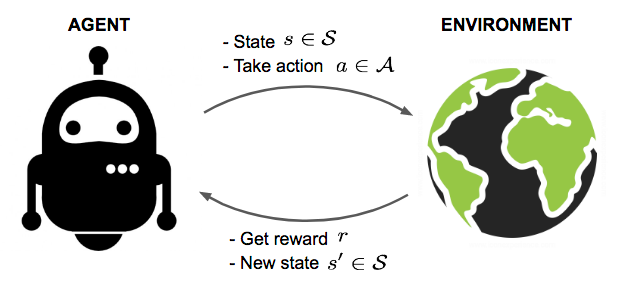
\includegraphics[scale=0.4]{images/RL_illustration.png}
    \caption{Simple scheme of a reinforcement learning system.}
    \label{fig:RL_illustration}
\end{figure}

\noindent
Reinforcement learning is divided in two approaches:
\begin{itemize}
    \item \textbf{Model-based}:
          The agent uses a transition model of the environment to help interpret the reward signals and to make decisions about how to act \cite{russell2021artificial}.
    \item \textbf{Model-free}:
          The agent learns the consequences of his actions through experience in order to refine his policy.
\end{itemize}

\noindent
Reinforcement learning algorithms are divided into several categories:
\begin{itemize}
    \item \textbf{Value-based}: Value-based methods are based on the estimation of a Value-function that estimate the value (expected return) of being in a given state according to a policy $\pi$,
    allowing you to choose the best action in each state.

    \item \textbf{Policy-search}: The policy-search approach describe a parametrized policy, which is often stochastic $\pi_{\theta}:(a | s)\rightarrow P[a | s]$, 
    and can be seen as an optimization problem where we need to find the best parameters $\theta$ to maximize
    a score function $J(\theta) = E_{\pi_\theta}[\sum \gamma r]$.
    
    \item \textbf{Actor-critic}: Actor-critic methods use both the value-based and policy-search approaches by combining value
    functions with an explicit representation of the policy.
\end{itemize}

\subsection{Q-Learning}
Q-learning \cite{watkins1992q} is a model-free reinforcement learning algorithm which estimate a value for each (state, action) pair
and with these estimated values compute a policy that can maximize the expected discounted reward.

Given a set of states S, a set of actions A, a policy $\pi : S \rightarrow A$ and a reward function $R : A \times S \rightarrow \mathbb{R}$, the algorithm assigns a quality value to each (state, action) pair using the quality function $Q : S \times A \rightarrow \mathbb{R}$, \cref{eq:qlearning}.
The quality values are updated iteratively at each agent action $a$ leading to a state $s'$ from a state $s$.
\begin{equation}
    Q(s, a) \leftarrow Q(s, a) + \alpha [R(s, a) + \gamma \max_a Q(s', a) - Q(s, a)]
    \label{eq:qlearning}
\end{equation}
%
where $\alpha \in [0, 1]$ is the learning rate and $\gamma \in [0, 1]$ is a discount factor which makes futures rewards less valuable than the current ones.

%The greedy policy $\pi(s) = \arg\max_a Q(s, a)$ is optimal when the Q values are accurate.

Given infinite exploration time the Q-learning algorithm is able to learn an optimal action-selection policy \cite{melo2001convergence}.

A problem of this method is the limitation of the state-action space required, that can be solved with an approximation function.
instead of storing each Q-values a mapping function could be learned to map a state-action pair to their respective Q-value.

\subsection{SARSA}
SARSA algorithm \cite{qiang2011reinforcement} is a variation of the Q-learning algorithm.
Its name come from $(s, a, r, s', a')$, that are (state, action, reward, next state, next action), and they are used to compute the update.

An algorithm has an ``Off-Policy'' technique if it learns the value function according to the action derived from another policy. On the other hand, it called ``On-Policy'' if it learns the value function according to the current action derived from the current policy.
Q-learning has an Off-Policy technique while SARSA has an On-Policy one.

The update formula of SARSA is similar to the one used by the Q-learning:
\begin{equation}
    Q(s, a) \leftarrow Q(s, a) + \alpha [R(s, a) + \gamma Q(s', a') - Q(s, a)]
\end{equation}
%
This means that SARSA updates the state based on the action taken, while Q-learning updates following the optimal policy.
Suppose to be in a ``cliff world'', where the agent has to walk from the starting cell to the goal cell along the edge of a cliff without falling off. Q-learning, following the optimal policy, would tend to be close to the edge of the cliff while SARSA would prefer a ``safer'' path.

\begin{figure}[ht]
    \centering
    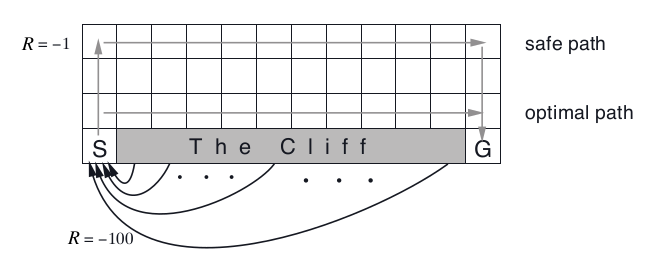
\includegraphics[scale=0.4]{images/cliff_word.png}
    \caption{Image to show the difference between SARSA and Q-learning in a ``cliff word''.}
\end{figure}

\section{Deep Reinforcement Learning}
\label{sec:drl}
When an MDP has a large number of states and actions, more memory and more time are required for learning.
To solve these problems it is possible to use approximation functions.
The function can be linear \cite{melo2008analysis} or non-linear as in the case of neural networks.

Deep reinforcement learning \cite{arulkumaran2017deep} combines reinforcement learning and deep learning and represents policies as a neural network.

The deep learning enables RL to scale to decision-making problems that were previously intractable \cite{arulkumaran2017deep}.
Instead of a manual engineering representation of the state space, deep RL can use a very large and unstructured input data.

A very big advantage that deep RL offers instead of other input representation,
is that it can handle unseen states well \cite{mnih2013playing} \cite{karpathy2016deep}.
This is because a large portion of pixels could be similar to an image already seen and on which the model has been trained, so the network is likely to produce a similar prediction to the image seen previously. Instead, algorithms like MDP behave randomly in these cases.

Despite the benefits of deep learning, reinforcement learning is known to be unstable or even to diverge when a nonlinear function approximator such as a neural network is used to represent the action-value (also known as Q) function \cite{mnih2015human}.
So new techniques were introduced to solve this instability.

\subsection{Deep Q-Network}
A Deep Q-Network (DQN) \cite{mnih2013playing} is a CNN adapted for RL used as a function approximator to estimate the Q-values,
where the inputs are images and the outputs depends on the number of actions.

A variant of Q-learning is used that combines experience replay and a target network in order to have a more stable target during training. 

The approximation of the Q-values is obtained by minimizing the following loss at each iteration $i$:
\begin{equation}
    L(\theta_i) = \mathbb{E}_{s, a, r, s'} [ ( y_i - Q(s, a; \theta_i))^2 ]
\end{equation}
where $y_i = r + \gamma \max_{a'} Q(s', a'; \theta_{i-1})$ is the target and $\theta$ are the network parameters.

Two networks are used: a Q-Network for estimating the Q-values and
a target network which is a snapshot of the network at the previous iteration with fixed parameters $\theta_{i- 1}$.
%
Experience replay collects transitions $(s, a, r, s')$ to a fixed-size buffer, called replay buffer, and during training 
compute the loss using a batch of transitions sampled from the buffer.
%
Thanks to these techniques, the DQNs were able to alleviate training instability and achieve remarkable performance.
